\chapter{Neural Language Modeling}

In this chapter, we introduce the notation used throughout the thesis and give a brief overview of the development of neural language modeling (NLM) since its inception. We also review some of the main weaknesses shown by this family of models and how they have been addressed in the literature. 

\todo{
	- Finish this (7-8 pages) \\
	- Mention CNN LMs ? \\
	- Softmax variants (hierarchical)? \\
	- Modern models (highway)? \\
	- Include references for n-grams? \\
	- Figures?
}

\section{Notation}
\label{sec:notation}

Before continuing, we will define the notation used in this thesis:

\begin{itemize}
	\item Scalars are denoted with lowercase letters, such as $x$.
	
	\item Vectors (of size $N$) are denoted with bold lowercase letters, such as $\mathbf{x}$ with its $i$-th element $\mathbf{x}_i$, and are always assumed to be column vectors.
	
	\item Matrices (of size $N \times M$) are denoted with uppercase letters, such as $X$ with $X_{ij}$ as its $(i,j)$-th element.
\end{itemize}

\section{Background}
\label{sec:background}

Prior to introducing the specifics of NLMs, we will formalize the task at hand and introduce some of its core concepts. 

\subsection{Language Modeling}

First, we define a \textbf{word-based language model} as a model able to compute the probability of a sentence or sequence words $P(w_1, \ldots ,w_n)$. Such models are of great use in tasks where we have to recognize words in noisy or ambiguous input such as speech recognition or machine translation, among others.

If now we decompose the joint probability of a sequence using the chain rule of probability as shown in \autoref{eq:lm}, we observe that the function that needs to be estimated boils down to the conditional probability of a word given the history of previous words. However, taking into account the whole context poses a problem as language is creative and any particular sequence might have occurred few (or no) times before.  Many of the models that we will introduce opt to approximate the real conditional distribution by making a Markov assumption as shown in \autoref{eq:markov}. This means that the probability of an upcoming word is fully characterized by the $n-1$ previous ones. Despite seeming an incorrect assumption for a complex source of information such as language, it has been proven to work really well in practice.

\begin{equation} \label{eq:lm}
	\begin{gathered}
		P(w_1, \ldots ,w_n)=P(w_1)P(w_2|w_1)P(w_3|w_{1}^{2}) \ldots P(w_n|w_{1}^{n-1}) \\
		= \prod_{k=1}^{n} P(w_k|w_{1}^{k-1})
	\end{gathered}
\end{equation}

\begin{equation} \label{eq:markov}
	P(w_k|w_{1}^{k-1}) \approx P(w_k|w_{k-1}^{k-n})
\end{equation}

\subsection{Evaluation}

Following a common practice in machine learning, we use a test set in order to evaluate our models. In the case of language modeling we have a word sequence $W_1^n=\{w_1, \ldots , w_n\}$ and the better the model is, the higher the probability it will assign to this sequence. Rather than working directly with raw probabilities we define a metric called \textbf{perplexity}, which is the geometric average of the inverse of the probability over the test set, as shown in \autoref{eq:pp}. Therefore, lower perplexity is better.

\begin{equation} \label{eq:pp}
	\begin{gathered}
		\text{Perplexity}(W_1^n) = P(W_1^n)^{-\frac{1}{n}} = \sqrt[n]{\frac{1}{P(W_1^n)}} \\
		= \sqrt[n]{\frac{1}{\prod_{k=1}^{n} P(w_k|W_{1}^{k-1})}}
	\end{gathered}
\end{equation}

Moreover, we can regard language as a source of information and apply the Information Theory toolbox to find a different (and equivalent) interpretation of perplexity. For that we need to introduce the basic concept of \textbf{entropy} (\autoref{eq:entropy} shows its formulation for discrete variables), which measures the expected uncertainty or ``surprise" $S$ of the value of a random variable $X$. Without going into details, it is easy to see that defining uncertainty as the negative logarithm (the specific base doesn't matter, but traditionally it is assumed to be 2) of the probability of each event matches our intuition (like $S(p)>S(q) \ \text{then} \ p<q$).

\begin{equation} \label{eq:entropy}
	H(X)=\mathbb{E}[S(X)]=-\sum_{x \in \mathcal{X}}P(x)\log_2(P(x)) \quad \text{with} \quad S(\cdot)=-\log_2(\cdot)
\end{equation}

A difference when it comes to language is that it involves dealing with sequences $W_1^n$ of discrete random variables. For a given language $L$ we can define the entropy of a variable ranging over all possible sequences of length $n$. To obtain the entropy-per-word we would only need to normalize by $n$ (\autoref{eq:entropySeq}).

\begin{equation} \label{eq:entropySeq}
	\frac{1}{n} H(W_1^n) = -\frac{1}{n}\sum_{W_1^n \in L}P(W_1^n)\log_2(P(W_1^n))
\end{equation}

However, in order to calculate the true entropy of a language we need to consider sequences of infinite length (\autoref{eq:trueEntropySeq}). Shannon-McMillan-Breiman theorem states that if the language is regular in certain ways we can take a single long enough sequence instead of summing over all possible sequences (* in \autoref{eq:trueEntropySeq}).

\begin{equation} \label{eq:trueEntropySeq}
	\begin{gathered}
		H(L) = -\lim\limits_{n \rightarrow \infty}\frac{1}{n}\sum_{W_1^n \in L}P(W_1^n)\log_2(P(W_1^n))\\
		\stackrel{*}{=} -\lim\limits_{n \rightarrow \infty}\frac{1}{n}\log_2(P(W_1^n))
	\end{gathered}
\end{equation}

Similarly we have \textbf{cross-entropy} which measures the relative entropy of $P$ with respect to $M$, $P$ being the true probability distribution and $M$ a model (e.g. an approximation) of $P$. After applying Shannon-McMillan-Breiman theorem and assuming that $n$ is large enough, we can see in \autoref{eq:crossEntropy} the final formulation of the cross-entropy, which is used as the default loss function when optimizing neural language models.

\begin{equation} \label{eq:crossEntropy}
	\begin{gathered}
		H(P,M) = -\lim\limits_{n \rightarrow \infty}\frac{1}{n}\sum_{W_1^n \in L}P(W_1^n)\log_2(M(W_1^n)) \\
		\stackrel{*}{=} -\lim\limits_{n \rightarrow \infty}\frac{1}{n}\log_2(M(W_1^n)) \approx -\frac{1}{n}\log_2(M(W_1^n)) \\
		= -\frac{1}{n}\sum_{k=1}^{n}\log_2(M(w_k|W_{1}^{k-1}))
	\end{gathered}
\end{equation}

Finally, we can see in \autoref{eq:relationCrossAndPP} how cross-entropy and perplexity are connected. This relation gives raise to a nice interpretation of perplexity as branching factor: entropy measures uncertainty (in bits, if we use $\log_2$) but in exponentiated form it's measured as the cardinality of a uniform distribution with equivalent uncertainty.

\begin{equation} \label{eq:relationCrossAndPP}
	\text{Perplexity}(W_1^n) = 2^{\text{cross-entropy}} = 2^{H(P,M)} = M(W_1^n)^{-\frac{1}{n}}
\end{equation}

\section{Feed-Forward Neural Language Models (FFNLM)}
\label{sec:forwardnlm}

Until the appearance of NLMs the most successful approaches were based on n-grams, which are Markov models that estimate words from a fixed window of previous
words and estimate probabilities by counting in a corpus and normalizing. Due to their nature n-gram estimates intrinsically suffer from sparsity and several methods like smoothing, backoff and interpolation have been proposed to deal with this problem.

Along those lines, the first successful attempt of applying neural networks \cite{bengio2003neural} raised the point that when modeling the joint distribution between many discrete random variables (such as words in a sentence), any change of these variables may have a drastic impact on the value of the estimated function. On the contrary, by using continuous variables we obtain better generalization because the function to be learned can be expected to have some local smoothness properties (``similar" words should get similar probabilities). While taking longer to train, this approach is able to achieve significantly better results by jointly learning word representations and a statistical language model.

\begin{figure}[H]
	\noindent\begin{minipage}{.4\linewidth}
		\centering
		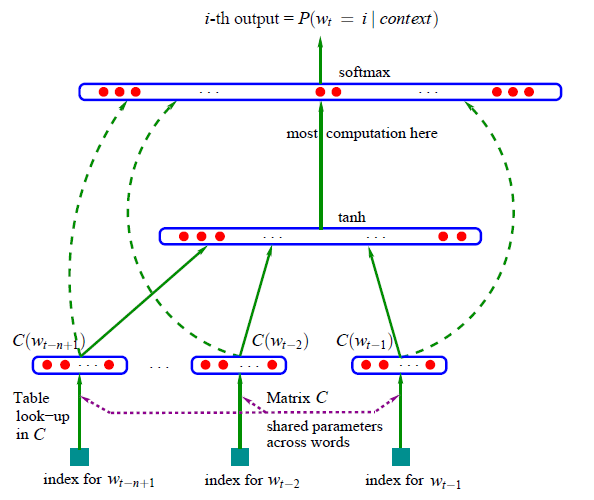
\includegraphics[scale=0.4]{fflm}
		\captionof{figure}{Feed-Forward NLM architecture}
		\label{fig:ffarch}
	\end{minipage}
	\hspace{0.25cm}
	\begin{minipage}{.7\linewidth}	
		\begin{equation} \label{eq:fwnlm}
		\openup 2ex
		\begin{gathered}
		\mathbf{x} = [C(w_{t-1}),C(w_{t-2}),\ldots,C(w_{t-n+1})] \\
		\mathbf{y} = W\mathbf{x} + U \tanh(H\mathbf{x}+\mathbf{d}) + \mathbf{b} \\
		P(w_t=i|w_{t-1},\ldots,w_{t-n+1}) = \frac{e^{\mathbf{y}_i}}{\sum_{n}e^{\mathbf{y}_n}} \\
		\end{gathered}
		\end{equation}
	\end{minipage}
\end{figure}

Similar to n-grams, the model introduced in \cite{bengio2003neural} conditions the probability of a word on the previous $n-1$ words. The main difference lies in the concept of ``distributed feature vectors"; words are embedded into a vector-space by assigning them a continuous real-vector representation. As seen in \autoref{fig:ffarch}, this is done via a look-up operation over the embedding matrix $C$. The concatenated word representations are then fed through one or more hidden layers and the resulting hidden representation is used to generate the unscaled log probabilities with a fully connected layer. Finally, a softmax operation produces a valid probability distribution over the full vocabulary.

\section{Word Vectors}
\label{sec:wv}

As we have seen in the previous section, distributed continuous vectors allow for ``clever" smoothing by taking into account automatically learnt syntactic and semantic features. \cite{mikolov2013efficient} picked up on this concept trying to find ways of training these vector representations more efficiently. The paper introduces a family of models known as \textbf{word2vec}, whose architecture matches the one from a FFNLM where the non-linear hidden layer has been removed (and we end up with a simple log bilinear model). The difference between them lies on the ``fake" objective (fake in the sense that we are only interested in the resulting embeddings and not the actual outputs of the model) they optimize for learning the word embeddings:

\begin{itemize}
	\item Continuous Bag-of-Words model (CBOW): given a symmetric window of size $k$ around a specific position $\{w_{i-k}, \ldots , w_{i-1}, w_{i+1}, \ldots w_{i+k}\}$ we want to predict that word $w_i$. The term ``bag-of-words" comes from the fact that the embeddings of the whole window are summed (instead of concatenated) and thus, order is not kept anymore.
	
	\item Continuous Skip-Gram model: given a specific position, we randomly sample words inside its surrounding window and try to predict them. Therefore, each training example is a tuple consisting of $w_i$ as input and a word from the window as output.
\end{itemize}

In addition to a simplified architecture and a modified objective, further optimizations for the Skip-Gram model were introduced in the follow-up paper \cite{mikolov2013distributed}. As we already saw in \autoref{eq:fwnlm}??, most of the computation is done in the softmax operation over the full vocabulary. In order to avoid this, we cast our task to a binary classification problem by making use of a new objective called \textbf{negative sampling}. Inspired by noise contrastive estimation (NCE), the task is to distinguish the target word $w_O$ from draws from a noise distribution $P_n(w)$ (e.g. unigram distribution) using logistic regression, where there are $k$ negative samples for each data sample (\autoref{eq:ns}).

\begin{equation} \label{eq:ns}
	\begin{gathered}
		\mathcal{L}(\theta) = \log(P(w_O|w_I))=\log(\sigma(\mathbf{v}_{w_O}^{\top} \mathbf{v}_{w_I})) + \sum_{i=1}^{k} \log(-\sigma(\mathbf{v}_{w_i}^{\top} \mathbf{v}_{w_I})) \\ 
		\text{with} \quad w_i \sim P_n(w)
	\end{gathered}
\end{equation}

Another famous family of word vectors is \textbf{GloVe} \cite{pennington2014glove}, where the objective is a weighted (weighting function $f(\cdot)$) least squares fit of the log-counts (\autoref{eq:glove}). Rather than taking a predictive model approach (like word2vec) to learn their vectors in order to improve their predictive ability, GloVe does dimensionality reduction on the co-occurrence counts matrix $N$. 

\begin{equation} \label{eq:glove}
	\mathcal{L}(\theta, N) = \sum_{i,j:N_{ij}>0}f(N_{ij})(\log(N_{ij})-(\mathbf{v}_{w_O}^{\top} \mathbf{v}_{w_I} + b_O + b_I))^2
\end{equation}

In summary, word vectors have become a standard in NLP and are used as input in all sorts of downstream tasks such as sentiment analysis.

\section{Recurrent Neural Language Models (RNNLM)}
\label{sec:lstm}

he \cite{hochreiter1997long} as in 

\noindent\begin{minipage}{.4\linewidth}
	\begin{equation} \label{eq:rnncell}
		\mathbf h_t = \sigma(W \mathbf x_t + U \mathbf h_{t-1})
	\end{equation}
\end{minipage}
\hspace{1cm}
\begin{minipage}{.5\linewidth}
	\begin{equation} \label{eq:lstmcell}
		\begin{gathered}
			\mathbf{f}_t = \sigma_g(W_f \mathbf{h}_{t-1} + U_f\mathbf{x}_t + \mathbf{b}_f) \\
			\mathbf{i}_t = \sigma_g(W_i \mathbf{h}_{t-1} + U_i \mathbf{x}_t + \mathbf{b}_i) \\
			\mathbf{o}_t = \sigma_g(W_o \mathbf{h}_{t-1} + U_o \mathbf{x}_t + \mathbf{b}_o) \\
			\mathbf{\tilde{c}}_t = \sigma_c(W_c \mathbf{h}_{t-1} + U_c \mathbf{x}_t + \mathbf{b}_c) \\
			\mathbf{c}_t = \mathbf{f}_{t} \odot \mathbf{c}_{t-1} + \mathbf{i}_{t} \odot \mathbf{\tilde{c}}_t \\
			\mathbf{h}_t = \mathbf{o}_{t} \odot \sigma_h(\mathbf{c}_{t})\\
		\end{gathered}
	\end{equation}
\end{minipage}
